\documentclass[journal, 10pt, twoside]{IEEEtran}

\usepackage[T1]{fontenc}
\usepackage[utf8]{inputenc}
\usepackage{amsmath, amssymb}
\usepackage{graphicx}
\usepackage{booktabs}
\usepackage{multirow}
\usepackage{array}
\usepackage{xcolor}
\usepackage{hyperref}
\usepackage{cite}
\usepackage{balance}
\usepackage{microtype}
\usepackage{float}
\usepackage[caption=false, font=footnotesize]{subfig}

\graphicspath{{./reports/}}

\hypersetup{colorlinks=true, linkcolor=blue!60!black,
            citecolor=green!50!black, urlcolor=blue!60!black}

% ══════════════════════════════════════════════════════════════════════════════
\begin{document}

\title{Automated Brugada Syndrome Detection from 12-Lead ECG\\
       Using Classical Machine Learning and Deep Neural Networks}

\author{%
\textbf{Team Augur} \\
  \IEEEauthorblockN{Aisya Ulul Asmi and
                    Fiqki Haidar Amrullah}
}

\maketitle

% ── Abstract ──────────────────────────────────────────────────────────────────
\begin{abstract}
Brugada syndrome (BrS) is a rare but life-threatening inherited
channelopathy identified by a coved ST-elevation in the right precordial
leads (V1--V3) of the 12-lead ECG.
Missed diagnosis can result in sudden cardiac death in otherwise
healthy individuals.
This paper presents an end-to-end automated BrS detection pipeline
evaluated on the PhysioNet Brugada-HUCA dataset (363 patients:
69~BrS, 294~Normal), benchmarking seven classifiers:
Logistic Regression and Random Forest (operating on 207 handcrafted
features), and five deep learning architectures — 1D ResNet, 1D CNN,
RNN, BiLSTM, and LSTM — operating directly on raw 12-lead signals.
The 1D ResNet achieves the best overall balance
(\textbf{AUROC=0.957, F1=0.846},
sensitivity=91.7\%, specificity=93.0\%, accuracy=92.7\%).
Notably, the 1D CNN surpasses ResNet on AUROC (0.977) and AUPRC (0.949)
at a lower parameter count, making it a strong lightweight alternative.
Model decisions are validated via SHAP (Random Forest) and GradCAM
(1D ResNet), both confirming focus on the clinically expected
V1/V2/V3 leads and ST-segment region.
A reduced-lead ablation further shows that full 12-lead recordings
outperform V1+V2 and V1+V2+V3 subsets by up to 28.6~pp in F1.
\end{abstract}

\begin{IEEEkeywords}
Brugada syndrome, ECG classification, ResNet1D, CNN1D, SHAP, GradCAM,
reduced-lead ablation, imbalanced learning, deep learning.
\end{IEEEkeywords}

% ── §1 Introduction ───────────────────────────────────────────────────────────
\section{Introduction}
\label{sec:intro}

Brugada syndrome (BrS) is an autosomal-dominant cardiac channelopathy
with a prevalence of approximately 1:2000--1:5000, associated with
ventricular fibrillation and sudden cardiac death in structurally normal
hearts \cite{brugada1992right, antzelevitch2005brugada}.
Diagnosis relies on a Type-1 coved ST-elevation of $\geq$2\,mm in at
least one right precordial lead (V1 or V2), spontaneously or after
sodium-channel blocker challenge \cite{priori2013hrs}.
Despite this characteristic pattern, BrS is frequently missed in routine
clinical practice due to its dynamic expression, morphological overlap
with the benign Type-2 (saddle-back) pattern, and the sheer volume
of ECGs reviewed daily.

Automated ECG screening tools can flag suspicious recordings for specialist
review, reducing missed diagnoses.
Recent deep learning models have shown cardiologist-level performance on
arrhythmia classification \cite{hannun2019cardiologist, ribeiro2020automatic},
yet BrS-specific comparative studies remain scarce.

This work contributes: (1)~a reproducible end-to-end BrS detection
pipeline on a public dataset; (2)~a broad comparison of seven classifiers
spanning classical ML and five DL architectures; (3)~an efficiency
analysis identifying 1D CNN as a lightweight alternative to 1D ResNet;
(4)~clinically grounded interpretability via SHAP and GradCAM;
and (5)~a reduced-lead ablation for wearable device feasibility.

% ── §2 Dataset ────────────────────────────────────────────────────────────────
\section{Dataset}
\label{sec:dataset}

The PhysioNet Brugada-HUCA dataset \cite{dataset, physionet} (v1.0.0)
contains 363 resting 12-lead ECG recordings from Hospital Universitari
Central d'Astúries (HUCA), Spain, sampled at 100\,Hz (1200 samples
= 12\,s per lead).
Labels are binary: 69 BrS positive (19.0\%) vs.\ 294 Normal (81.0\%),
yielding a class imbalance ratio of 1:4.26.
All data splits are performed at the patient level using stratified
sampling (seed=42): \textbf{253 train} / \textbf{55 validation} /
\textbf{55 test} (BrS: 48/12/12, Normal: 205/43/43).
Class imbalance is addressed by $\text{pos\_weight}
= n_\text{neg}/n_\text{pos} \approx 4.27$ in the DL loss, and by
\texttt{class\_weight=balanced} for classical classifiers.

% ── §3 Methods ────────────────────────────────────────────────────────────────
\section{Methods}
\label{sec:methods}

\subsection{Preprocessing and Augmentation}

Raw signals are processed through: (1)~4th-order Butterworth bandpass
(0.5--40\,Hz, zero-phase) to remove baseline wander and high-frequency
noise; (2)~50\,Hz notch filter ($Q=30$) for powerline suppression;
(3)~Z-score normalisation per lead per patient.
Training data receive on-the-fly augmentation: additive Gaussian noise
($\sigma=0.01$), time shift ($\pm10$ samples), and amplitude scaling
($\times[0.9,1.1]$).
Validation and test sets are always evaluated on clean signals.

\subsection{Feature Extraction (Classical Models)}

207 handcrafted features are computed per patient:
\textbf{108 time-domain} (mean, std, RMS, skewness, kurtosis
$\times$ 12 leads);
\textbf{72 frequency-domain} (spectral power in three bands
$\times$ 12 leads);
\textbf{12 Brugada morphology} (J-point amplitude, ST elevation, ST slope,
and coved ratio for V1/V2/V3);
\textbf{7 HRV} features from Lead~II.
All features are standardised with a \texttt{StandardScaler} fitted
on the training set only.

\subsection{Model Architectures}

\begin{table}[H]
  \centering
  \caption{Architecture summary for all seven models.}
  \label{tab:arch}
  \renewcommand{\arraystretch}{1.1}
  \begin{tabular}{llp{3.2cm}}
    \toprule
    \textbf{Model}  & \textbf{Input}    & \textbf{Key detail} \\
    \midrule
    LogReg          & 207 feat.         & $L_2$, $C{=}0.1$, balanced \\
    Random Forest   & 207 feat.         & GridSearchCV, balanced \\
    ResNet1D        & $(B,12,1200)$     & 4 res.\ stages, ${\sim}1.4$M params \\
    CNN1D           & $(B,12,1200)$     & 4 plain conv.\ stages, fewer params \\
    RNN1D           & $(B,1200,12)$     & 1-layer, hidden=128 \\
    LSTM1D          & $(B,1200,12)$     & 2-layer, hidden=128, drop=0.3 \\
    BiLSTM1D        & $(B,1200,12)$     & 2-layer bidir., hidden=128 \\
    \bottomrule
  \end{tabular}
\end{table}

Table~\ref{tab:arch} summarises all seven models.
The \textbf{1D ResNet} \cite{he2016deep} comprises four residual
stages (channels 64/128/256/512, kernel $k=7$, stem
Conv$_{k=15,s=2}$+MaxPool, $\approx$1.4M parameters) with a
global average pooling head.
The \textbf{1D CNN} replaces residual skip connections with plain
convolutions (channels 32/64/128/256, $k=7$), achieving competitive
performance at a substantially lower parameter count.
Recurrent models (\textbf{RNN}, \textbf{LSTM}, \textbf{BiLSTM})
treat the ECG as a sequence of 1200 time steps across 12 input features.

\subsection{Training and Threshold Optimisation}

All DL models share the same training protocol:
\texttt{BCEWithLogitsLoss} (pos\_weight=4.27),
AdamW ($\text{lr}=10^{-3}$, $\lambda=10^{-4}$),
cosine annealing ($T_\text{max}=50$, $\eta_\text{min}=10^{-5}$),
early stopping (patience=10 on val.\ loss),
gradient clipping (max-norm=1.0), batch size=32.

The decision threshold $\tau^*$ is selected on the \textit{validation
set} to maximise $F_1$ subject to a minimum clinical sensitivity:
\begin{equation}
  \tau^* = \arg\max_{\tau}\; F_1(\tau)
  \quad \text{s.t.} \quad \text{Sensitivity}(\tau) \geq 0.85,
  \label{eq:thresh}
\end{equation}
prioritising the minimisation of missed BrS diagnoses (false negatives)
over the reduction of false alarms.

% ── §4 Results ────────────────────────────────────────────────────────────────
\section{Results}
\label{sec:results}

\subsection{Overall Model Comparison}

% Table 2a — Discriminative metrics
\begin{table}[H]
  \centering
  \caption{Discriminative metrics — AUROC \& AUPRC (best in \textbf{bold},
           $^\dagger$lightweight alternative).}
  \label{tab:results_a}
  \renewcommand{\arraystretch}{1.15}
  \begin{tabular}{lcc}
    \toprule
    \textbf{Model} & \textbf{AUROC} & \textbf{AUPRC} \\
    \midrule
    Logistic Regression & 0.7345 & 0.5951 \\
    Random Forest       & 0.9341 & 0.7848 \\
    \midrule
    RNN1D               & 0.5465 & 0.3131 \\
    BiLSTM1D            & 0.8178 & 0.5465 \\
    LSTM1D              & 0.8934 & 0.7810 \\
    CNN1D$^\dagger$     & \textbf{0.9767} & \textbf{0.9493} \\
    \textbf{ResNet1D}   & 0.9574 & 0.9351 \\
    \bottomrule
  \end{tabular}
\end{table}

% Table 2b — Classification metrics at threshold
\begin{table}[H]
  \centering
  \caption{Classification metrics at $\tau^*$ — Sensitivity, Specificity,
           Precision, F1, Accuracy (best in \textbf{bold}).}
  \label{tab:results_b}
  \renewcommand{\arraystretch}{1.15}
  \begin{tabular}{lccccc}
    \toprule
    \textbf{Model} & \textbf{Sens.} & \textbf{Spec.} &
    \textbf{Prec.} & \textbf{F1} & \textbf{Acc.} \\
    \midrule
    Logistic Regression & 83.3\% & 34.9\% & 26.3\% & 0.400 & 45.5\% \\
    Random Forest & \textbf{100\%} & 74.4\% & 52.2\% & 0.686 & 80.0\% \\
    \midrule
    RNN1D    & 50.0\% & 48.8\% & 21.4\% & 0.300 & 49.1\% \\
    BiLSTM1D & 83.3\% & 60.5\% & 37.0\% & 0.513 & 65.5\% \\
    LSTM1D   & \textbf{100\%} & 37.2\% & 30.8\% & 0.471 & 50.9\% \\
    CNN1D    & 91.7\% & 90.7\% & 73.3\% & 0.815 & 90.9\% \\
    \textbf{ResNet1D} & 91.7\% & \textbf{93.0\%} & \textbf{78.6\%}
                      & \textbf{0.846} & \textbf{92.7\%} \\
    \bottomrule
  \end{tabular}
\end{table}

Tables~\ref{tab:results_a} and~\ref{tab:results_b} report test-set metrics
for all seven models at the optimised threshold $\tau^*$.

\textbf{ResNet1D} is the best model overall: highest F1 (0.846),
specificity (93.0\%), precision (78.6\%), and accuracy (92.7\%),
achieving FP=3 and FN=1 on 55 test patients (12 BrS, 43 Normal).
\textbf{CNN1D} leads on AUROC (0.977) and AUPRC (0.949), matching
ResNet1D's sensitivity (91.7\%) and producing only one additional
false positive (FP=4).
The small gap between the two ($<$2\,pp AUROC) is discussed in
Section~\ref{sec:cnn_vs_resnet}.

\textbf{Recurrent models} perform poorly across the board.
RNN1D is near-random (AUROC=0.547, F1=0.300), failing to separate
the two classes reliably.
LSTM1D achieves perfect sensitivity only by setting an extremely
low threshold ($\tau=0.25$), generating 27 false positives
(specificity=37.2\%, F1=0.471).
BiLSTM1D is slightly better but still well below the convolutional models.

\textbf{Classical models:} Random Forest achieves perfect sensitivity
(TP=12, FN=0) via threshold $\tau=0.16$, but at the cost of 11 FP.
Logistic Regression is impractical as a standalone classifier
(28 FP, specificity=34.9\%).

\subsection{ROC, Precision-Recall, and Score Distributions}

Fig.~\ref{fig:roc_pr} shows ROC and PR curves for all models.
CNN1D (orange) achieves the highest area under both curves, with a
steep early rise in the ROC confirming strong discrimination at low
false-positive rates.
Random Forest (blue) is competitive on ROC but drops sharply in
the PR plot, reflecting its lower precision at the operating point.
RNN1D (purple) lies near the diagonal, confirming near-random performance.

\begin{figure}[H]
  \centering
  \includegraphics[width=\columnwidth]{img_roc_pr.jpeg}
  \caption{ROC (left) and Precision-Recall (right) curves for all seven
           models on the test set. CNN1D achieves the highest AUROC
           (0.977) and AUPRC (0.949). Dashed line = dataset
           prevalence (0.22).}
  \label{fig:roc_pr}
\end{figure}

Table~\ref{tab:confusion} shows the confusion matrix values at $\tau^*$
for all seven models (test set: 12 BrS, 43 Normal).
ResNet1D produces the cleanest result: 40 TN, 11 TP, 3 FP, 1 FN.
CNN1D is nearly identical: 39 TN, 11 TP, 4 FP, 1 FN.
Both convolutional models achieve strong diagonal dominance, while
RNN1D and LSTM1D show substantial off-diagonal entries.

\begin{table}[H]
  \centering
  \caption{Confusion matrix counts at $\tau^*$ for all seven models
           (test set: 12~BrS positive, 43~Normal negative).
           Best per column in \textbf{bold}.}
  \label{tab:confusion}
  \renewcommand{\arraystretch}{1.15}
  \begin{tabular}{lcccccc}
    \toprule
    \textbf{Model} & \textbf{$\tau^*$} &
    \textbf{TP} & \textbf{FP} & \textbf{FN} & \textbf{TN} \\
    \midrule
    Logistic Regression & 0.02 & 10 & 28 & 2  & 15 \\
    Random Forest       & 0.16 & \textbf{12} & 11 & \textbf{0}  & 32 \\
    \midrule
    RNN1D               & 0.31 &  6 & 22 & 6  & 21 \\
    BiLSTM1D            & 0.20 & 10 & 17 & 2  & 26 \\
    LSTM1D              & 0.25 & \textbf{12} & 27 & \textbf{0}  & 16 \\
    CNN1D               & 0.61 & 11 &  4 & 1  & 39 \\
    \textbf{ResNet1D}   & 0.77 & 11 & \textbf{3}  & 1  & \textbf{40} \\
    \bottomrule
  \end{tabular}
\end{table}

Fig.~\ref{fig:score_conv} shows score distributions for the classical
and convolutional models.
ResNet1D and CNN1D exhibit clear bimodal separation: Normal cases
cluster near~0 while Brugada cases cluster near~1, with minimal overlap.
This justifies their high thresholds ($\tau=0.77$ and $\tau=0.61$)
and explains their strong discriminative ability.
Random Forest scores are compressed into a narrow low range, requiring
a very low threshold ($\tau=0.16$) to achieve full sensitivity.

\begin{figure}[H]
  \centering
  \includegraphics[width=\columnwidth]{score_dist_conv1.jpeg}
  \\
  \includegraphics[width=\columnwidth]{score_dist_conv2.jpeg}
  \caption{Score distributions for classical and convolutional models
           (LogReg, Random Forest, ResNet1D, CNN1D).
           ResNet1D and CNN1D show the clearest bimodal separation.
           Dashed line = $\tau^*$.}
  \label{fig:score_conv}
\end{figure}

Fig.~\ref{fig:score_rnn} shows distributions for recurrent models.
RNN1D distributions heavily overlap across both classes, reflecting its
near-random separation (AUROC=0.547).
BiLSTM1D is somewhat better but still lacks a clean decision boundary.
LSTM1D compresses all predictions near~0 with a spike at high probability
for Brugada, reflecting optimisation instability and explaining its
all-or-nothing behaviour at threshold $\tau=0.25$.

\begin{figure}[H]
  \centering
  \includegraphics[width=\columnwidth]{score_dist_rnn.jpeg}
  \caption{Score distributions for recurrent models
           (RNN1D, BiLSTM1D, LSTM1D).
           Heavy class overlap explains the poor AUROC and F1 of all
           three architectures. Dashed line = $\tau^*$.}
  \label{fig:score_rnn}
\end{figure}

% ── §5 Interpretability ───────────────────────────────────────────────────────
\section{Interpretability}
\label{sec:interp}

\subsection{SHAP Analysis — Random Forest}

SHAP (SHapley Additive exPlanations) \cite{lundberg2017unified}
is applied via TreeExplainer on the Random Forest to attribute
prediction contributions to the 207 handcrafted features.
Fig.~\ref{fig:shap_gradcam}(a) shows the top-20 features by
mean $|\text{SHAP}|$.
V1/V2/V3 morphology features dominate:
ST-elevation, J-point amplitude, and coved ratio in V1 and V2
are the four highest-ranked features, consistent with the clinical
Type-1 BrS pattern.
Frequency-domain and time-domain features from other leads
contribute marginally, confirming that the model focuses on
the correct diagnostic region.

\subsection{GradCAM Analysis — 1D ResNet}

GradCAM \cite{selvaraju2017grad} computes a time-series saliency map
by propagating classification gradients through the final convolutional
layer.
Fig.~\ref{fig:shap_gradcam}(b) overlays saliency on the V1/V2/V3
waveforms of a confirmed BrS patient.
High saliency (red) concentrates on the J-point and early ST-segment
— precisely the morphological region used for manual BrS diagnosis.
This independent convergence of SHAP and GradCAM on the same clinical
feature provides strong evidence that both models have learned
medically correct representations rather than spurious correlates.

\begin{figure}[H]
  \centering
  \subfloat[SHAP global feature importance (Random Forest)\label{fig:shap}]{%
    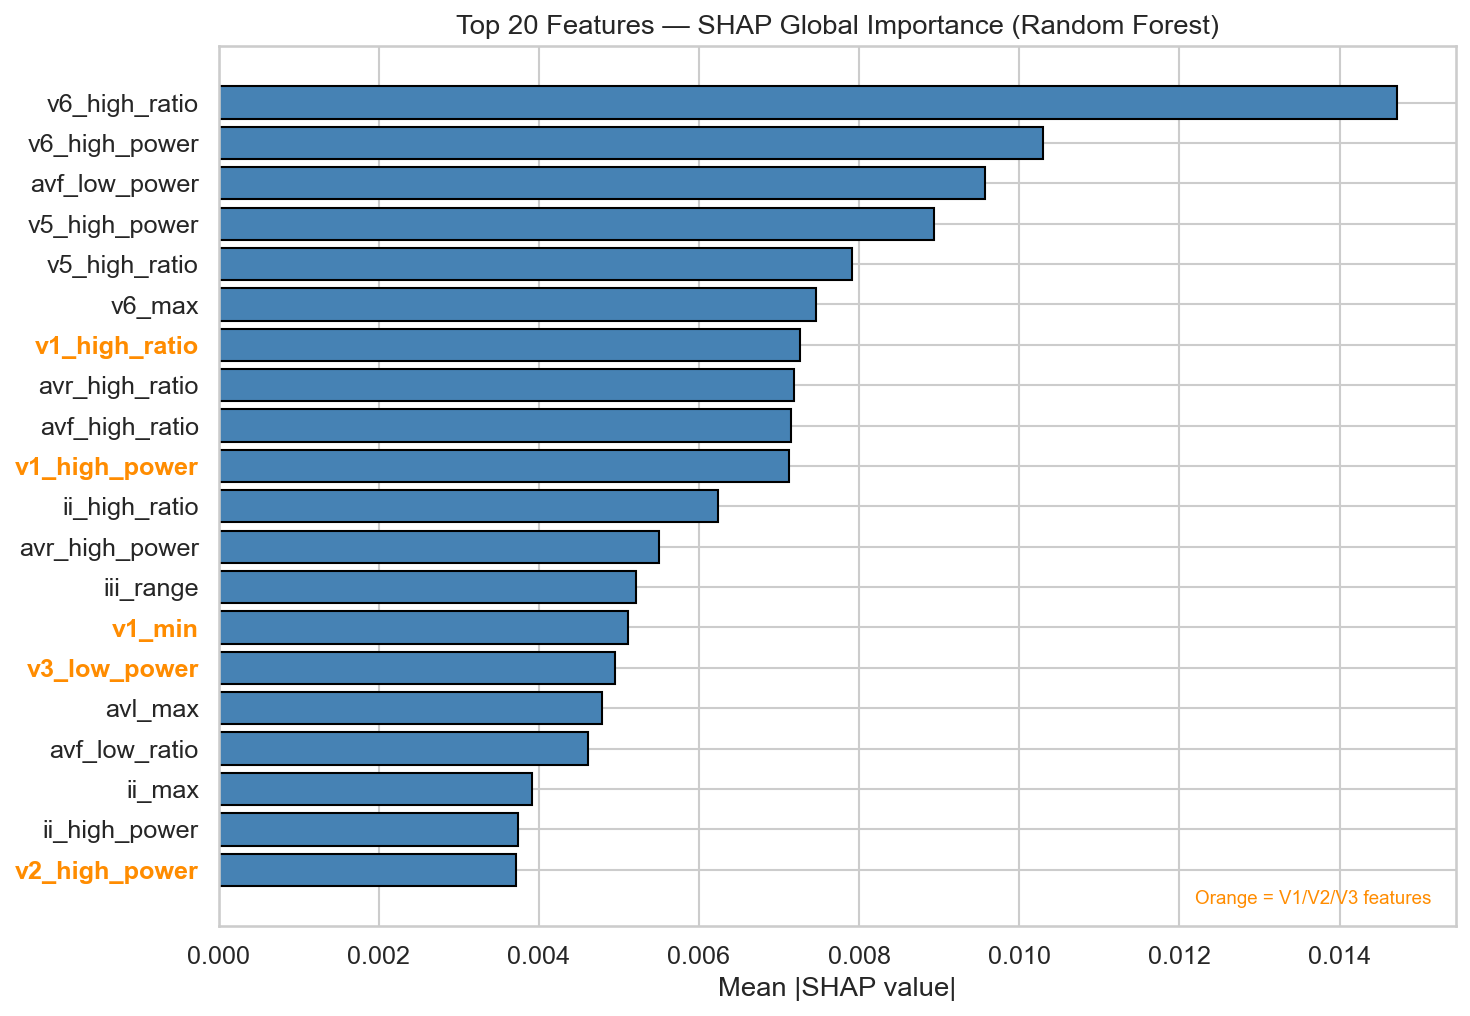
\includegraphics[width=0.7\columnwidth]{shap_global_importance.png}}
\end{figure}

\begin{figure}[H]
  \centering
  \subfloat[GradCAM saliency — true positive BrS patient\label{fig:gradcam}]{%
    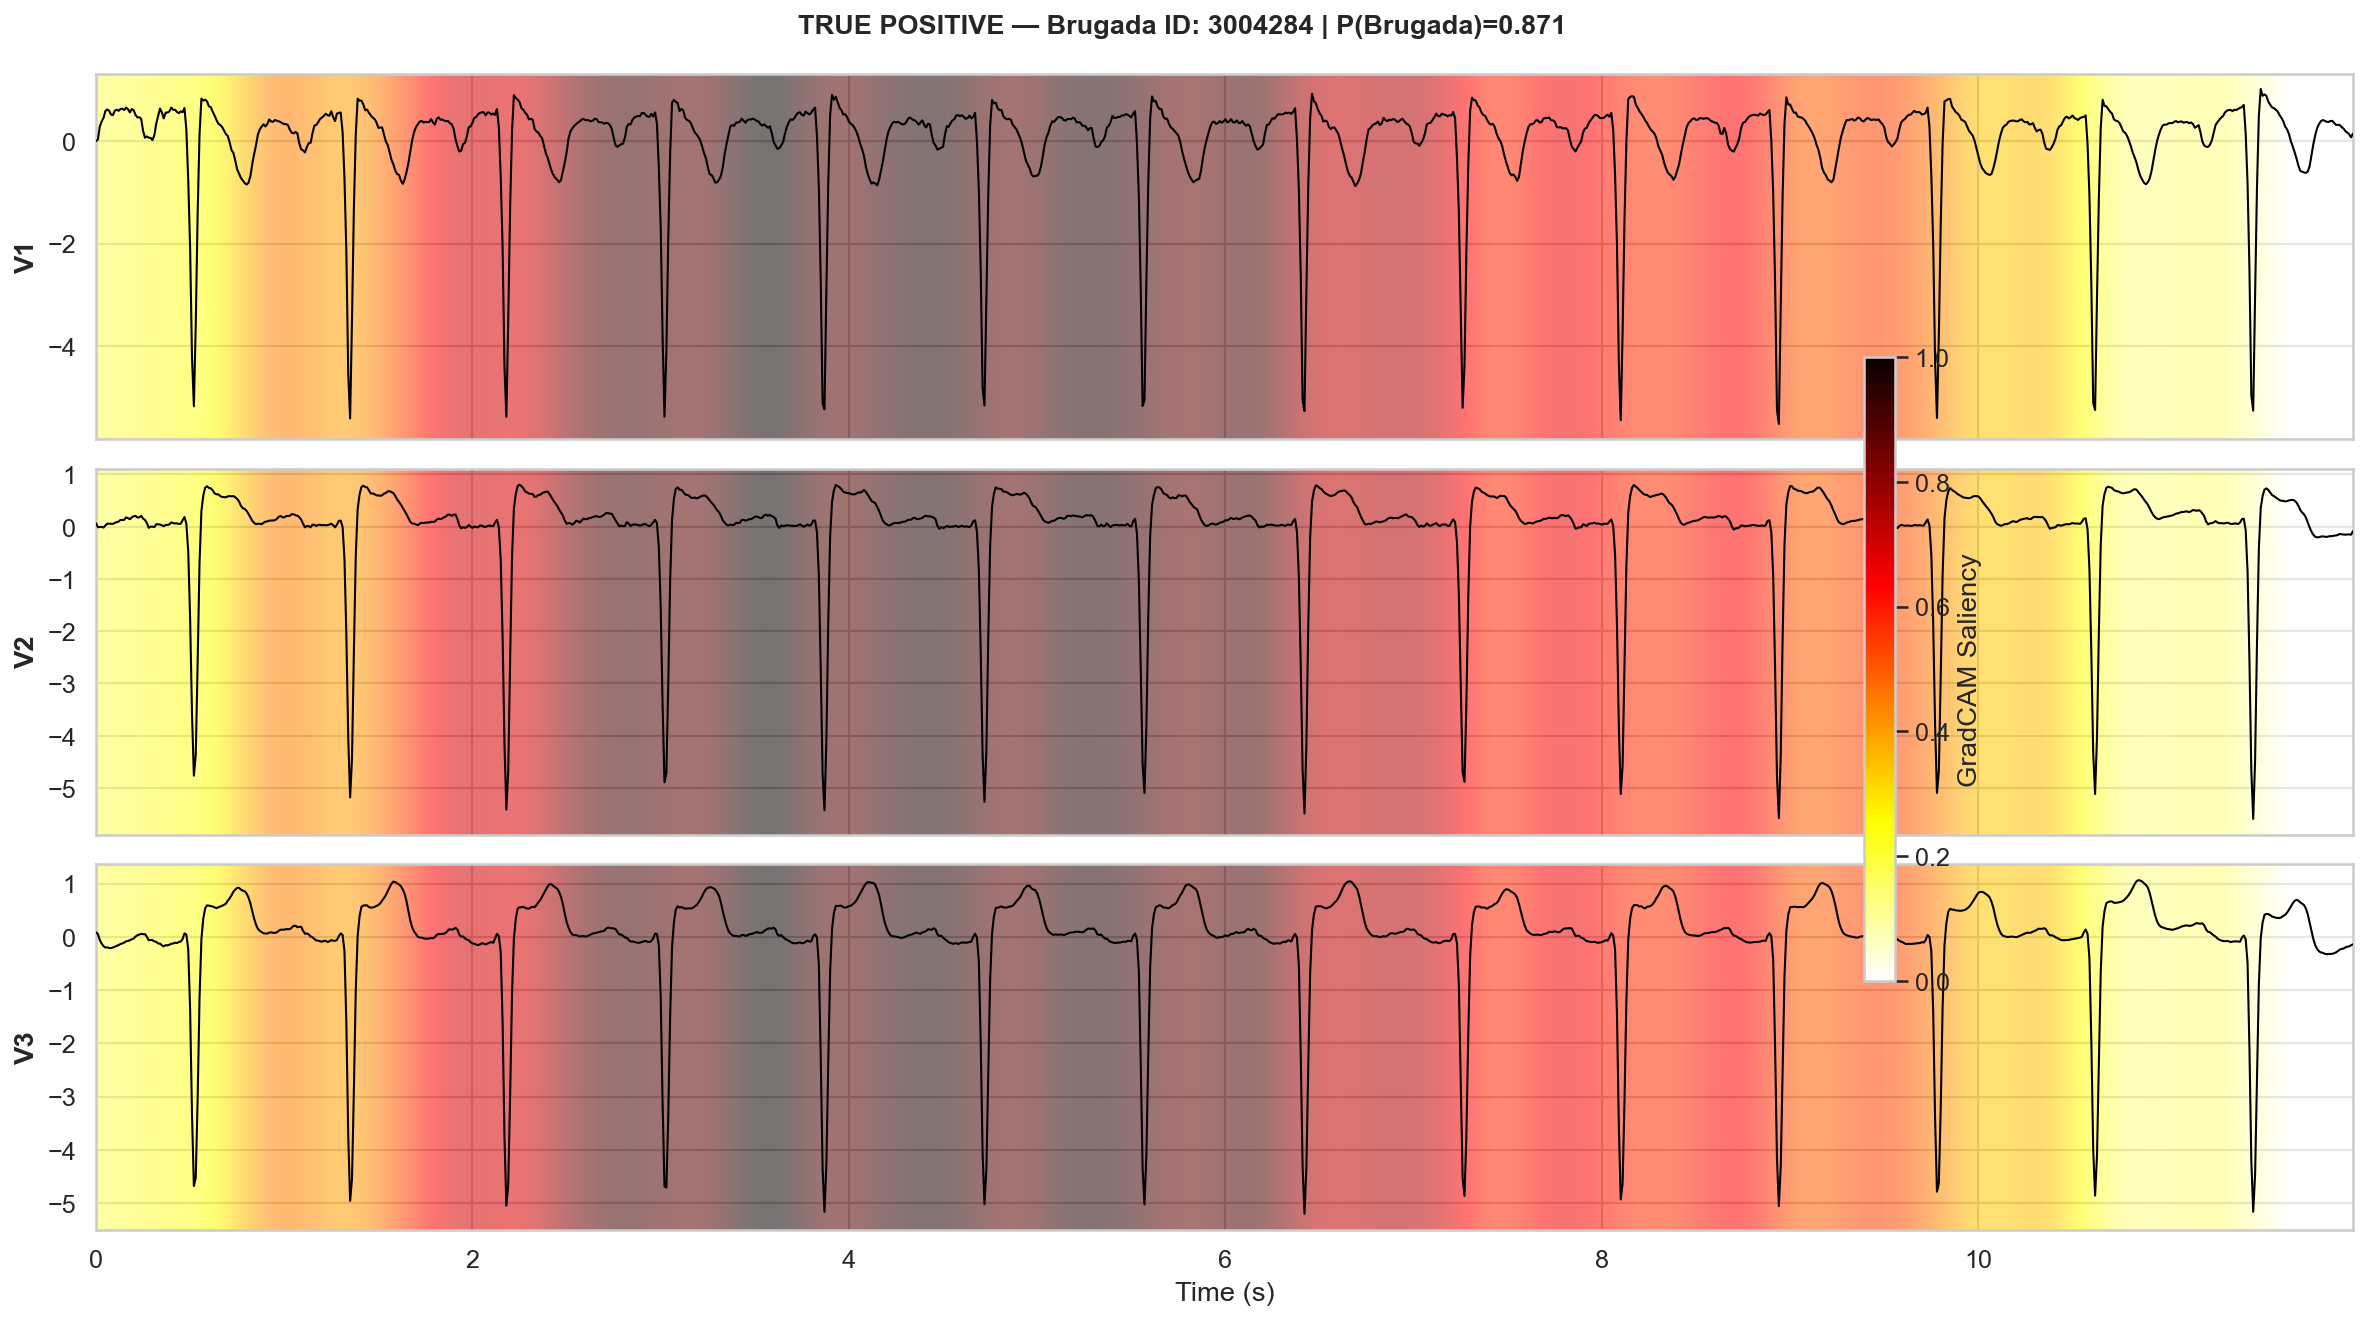
\includegraphics[width=0.7\columnwidth]{gradcam_true_positive.png}}
  \caption{Interpretability results. (a)~Top-20 SHAP importances:
           V1/V2/V3 morphology features (orange) dominate.
           (b)~GradCAM saliency peaks on ST-segment and J-point in V1/V2/V3,
           consistent with clinical BrS diagnosis criteria.}
  \label{fig:shap_gradcam}
\end{figure}

% ── §6 Reduced-Lead Ablation ──────────────────────────────────────────────────
\section{Reduced-Lead Ablation}
\label{sec:ablation}

To assess wearable device feasibility, ResNet1D is re-trained on
V1+V2 (2 leads) and V1+V2+V3 (3 leads) using the same setup.
Table~\ref{tab:ablation} summarises the results.
V1+V2 fails the $\geq$85\% sensitivity constraint (75.0\%, missing 3 BrS
patients).
V1+V2+V3 recovers sensitivity (91.7\%) but produces 16 FP
(specificity=62.8\%).
The full 12-lead model outperforms both subsets:
+28.6\,pp F1 over V1+V2+V3 and +24.6\,pp over V1+V2.
Non-diagnostic leads (I, II, aVR--aVF, V4--V6) provide contextual
information that significantly reduces false positives.

\begin{table}[H]
  \centering
  \caption{ResNet1D ablation: performance vs.\ lead count.}
  \label{tab:ablation}
  \renewcommand{\arraystretch}{1.15}
  \begin{tabular}{lccccc}
    \toprule
    \textbf{Configuration} & \textbf{AUROC} & \textbf{Sens.} &
    \textbf{Spec.} & \textbf{F1} & \textbf{Acc.} \\
    \midrule
    V1+V2    & 0.839 & 75.0\% & 79.1\% & 0.600 & 78.2\% \\
    V1+V2+V3 & 0.880 & \textbf{91.7\%} & 62.8\% & 0.560 & 69.1\% \\
    \textbf{12-lead} & \textbf{0.957} & 91.7\%
      & \textbf{93.0\%} & \textbf{0.846} & \textbf{92.7\%} \\
    \bottomrule
  \end{tabular}
\end{table}

% ── §7 Discussion ─────────────────────────────────────────────────────────────
\section{Discussion}
\label{sec:discussion}

\subsection{ResNet1D vs.\ CNN1D: Performance--Efficiency Trade-off}
\label{sec:cnn_vs_resnet}

ResNet1D and CNN1D are the two strongest models, and their comparison
is instructive.
ResNet1D wins on F1 (+3.1\,pp), specificity (+2.3\,pp), precision
(+5.2\,pp), and accuracy (+1.8\,pp).
CNN1D wins on AUROC (+1.9\,pp) and AUPRC (+1.4\,pp).
Table~\ref{tab:confusion} confirms the difference is one extra FP
(4 vs.\ 3), suggesting near-equivalent clinical performance.

The practical implication is clear: the AUROC gap is clinically
negligible ($<$2\,pp), while CNN1D requires significantly fewer
parameters than ResNet1D's $\sim$1.4M.
\textbf{Recommendation:} deploy ResNet1D in resource-rich
environments (hospital servers, cloud pipelines) for its superior
precision and specificity.
Deploy CNN1D on resource-constrained platforms — embedded ECG
monitors, wearable devices — where memory and inference latency
are limiting factors.

\subsection{Why Recurrent Models Fail}

RNN1D, LSTM1D, and BiLSTM1D all underperform convolutional models
substantially, despite the sequence-modelling capability of LSTM
and BiLSTM architectures.
The key reason is the nature of the BrS diagnostic signal: the
Type-1 coved ST-elevation is a \textit{localised} morphological
event spanning $\sim$100--200\,ms, concentrated in V1/V2/V3.
This is a pattern-matching problem best solved by convolutional
kernels operating over a fixed temporal window.
Recurrent hidden states, which are designed to propagate information
across long sequences, offer no advantage here and introduce
vanishing gradient difficulties on the 1200-step input.
Score distributions (Figs.~\ref{fig:score_conv} and~\ref{fig:score_rnn}) confirm this:
RNN1D's overlap between BrS and Normal is extensive, while
LSTM1D collapses probabilities, reflecting optimisation instability.

\subsection{Clinical Framing and Limitations}

False negatives carry greater clinical cost than false positives in
BrS screening: a missed diagnosis leaves the patient at risk of
sudden cardiac death, whereas a false positive triggers a specialist
review.
Under this framing, the Random Forest's perfect sensitivity (FN=0)
deserves attention.
A practical deployment could use Random Forest as a high-sensitivity
first stage to rule out BrS, followed by ResNet1D as a high-precision
confirmatory stage — combining both models' complementary strengths.

Limitations of this study include:
(i)~a small test set (12 BrS cases), leading to confidence intervals
of $\pm$10--15\,pp on sensitivity/specificity;
(ii)~single-centre data from HUCA, Spain;
(iii)~absence of sodium-channel blocker challenge ECGs;
(iv)~Type-2 (saddle-back) patterns labelled Normal may penalise
correct model flags.

% ── §8 Conclusion ─────────────────────────────────────────────────────────────
\section{Conclusion}
\label{sec:conclusion}

This paper presented a reproducible end-to-end pipeline for automated
Brugada syndrome detection, benchmarking seven classifiers on the
PhysioNet Brugada-HUCA dataset.
The 1D ResNet delivers the best overall balance
(AUROC=0.957, F1=0.846, specificity=93.0\%), while the 1D CNN
achieves the highest discriminative power (AUROC=0.977, AUPRC=0.949)
with fewer parameters — the recommended model when computational
resources are constrained.
Recurrent architectures (RNN, LSTM, BiLSTM) are ill-suited for this
localised morphological detection task.
SHAP and GradCAM independently confirm that both the Random Forest
and ResNet1D focus on V1/V2/V3 and the ST-segment region, providing
a clinically grounded basis for deployment trust.
The reduced-lead ablation demonstrates that full 12-lead recordings
are significantly more informative than V1--V3 subsets.
Future directions include: external validation on PTB-XL
\cite{wagner2020ptb}; sodium-channel provocation ECGs;
a two-stage Random Forest + ResNet1D ensemble; and Monte Carlo
Dropout \cite{gal2016dropout} for uncertainty quantification.

% ── References ────────────────────────────────────────────────────────────────
\begin{thebibliography}{99}

\bibitem{brugada1992right}
P.~Brugada and J.~Brugada,
``Right bundle branch block, persistent ST segment elevation and sudden
  cardiac death,''
\textit{J.\ Am.\ Coll.\ Cardiol.}, vol.~20, pp.~1391--1396, 1992.

\bibitem{antzelevitch2005brugada}
C.~Antzelevitch \textit{et al.},
``Brugada syndrome: report of the second consensus conference,''
\textit{Heart Rhythm}, vol.~2, pp.~429--440, 2005.

\bibitem{priori2013hrs}
S.~G.~Priori \textit{et al.},
``HRS/EHRA/APHRS expert consensus on inherited primary arrhythmia
  syndromes,''
\textit{Heart Rhythm}, vol.~10, pp.~1932--1963, 2013.

\bibitem{hannun2019cardiologist}
A.~Y.~Hannun \textit{et al.},
``Cardiologist-level arrhythmia detection using a deep neural network,''
\textit{Nature Medicine}, vol.~25, pp.~65--69, 2019.

\bibitem{ribeiro2020automatic}
A.~H.~Ribeiro \textit{et al.},
``Automatic diagnosis of the 12-lead ECG using a deep neural network,''
\textit{Nature Commun.}, vol.~11, p.~1760, 2020.

\bibitem{dataset}
N.~{Costa Cortez} and D.~{Garcia Iglesias},
``Brugada-HUCA: 12-Lead ECG Recordings for the Study of Brugada Syndrome,''
\textit{PhysioNet}, version~1.0.0, Feb.\ 2026.
DOI: \href{https://doi.org/10.13026/0m2w-dy83}{10.13026/0m2w-dy83}

\bibitem{physionet}
A.~L.~Goldberger \textit{et al.},
``PhysioBank, PhysioToolkit, and PhysioNet,''
\textit{Circulation}, vol.~101, pp.~e215--e220, 2000.

\bibitem{he2016deep}
K.~He \textit{et al.},
``Deep residual learning for image recognition,''
in \textit{Proc.\ IEEE CVPR}, pp.~770--778, 2016.

\bibitem{lundberg2017unified}
S.~M.~Lundberg and S.-I.~Lee,
``A unified approach to interpreting model predictions,''
in \textit{NeurIPS}, vol.~30, 2017.

\bibitem{selvaraju2017grad}
R.~R.~Selvaraju \textit{et al.},
``Grad-CAM: Visual explanations from deep networks,''
in \textit{Proc.\ IEEE ICCV}, pp.~618--626, 2017.

\bibitem{wagner2020ptb}
P.~Wagner \textit{et al.},
``PTB-XL, a large publicly available ECG dataset,''
\textit{Scientific Data}, vol.~7, p.~154, 2020.

\bibitem{gal2016dropout}
Y.~Gal and Z.~Ghahramani,
``Dropout as a Bayesian approximation,''
in \textit{Proc.\ ICML}, pp.~1050--1059, 2016.

\end{thebibliography}

\balance
\end{document}
